\section{Lecture -- Week 4}

\subsection{The symmetric group}

\index{Cycle}
Let $\sigma\in\Sym_n$. We say that the permutation $\sigma$ is an $r$-cycle 
if there are $a_1,\dots,a_r\in\{1,\dots,n\}$ such that 
$\sigma(j)=j$ for all $j\not\in\{a_1,\dots,a_r\}$ and 
\[
\sigma(a_i)=\begin{cases}
a_{i+1} & \text{if $i<r$},\\
a_1 & \text{if $i=r$}.
\end{cases}
\]

For example, $(12)$, $(13)$ and $(23)$ are 2-cycles of 
$\Sym_3$. Note that 
2-cycles are called \emph{transpositions}.
The permutations $(123)$ and $(132)$ are 3-cycles of $\Sym_3$.

\index{Disjoint permutations}
We say that the permutations $\sigma,\tau\in\Sym_n$ 
are \emph{disjoint} if for all 
$j\in\{1,\dots,n\}$
one has $\sigma(j)=j$ or $\tau(j)=j$. For example, 
$(134)$ and $(25)$ are disjoint. The permutations $(134)$ and 
$(24)$ are not disjoint. 

If $\sigma\in\Sym_n$ and $j$ is such that 
$\sigma(j)=j$, then $j$ is a fixed point of $\sigma$. The elements 
$j$ such that 
$\sigma(j)\ne j$ are the points moved by 
$\sigma$.

\begin{claim}
Disjoint permutations commute. 
\end{claim}


We now prove that every permutation can be written 
as product of disjoint cycles. 
The decomposition is unique up to the order of the factors. 
We start with a lemma (used to prove the uniqueness of the decomposition).

\begin{lemma}
        Let $\sigma=\alpha\beta\in\Sym_n$ with $\alpha$ and $\beta$ disjoint permutations. If $\alpha(
i)\ne i$, then $\sigma^k(i)=\alpha^k(i)$ for all $k\geq0$.
\end{lemma}

\begin{proof}
    Without loss of generality, we may assume that $k>0$. 
    Let $i\in\{1,\dots,n\}$. Then \[
    \sigma^k(i)=(\alpha\beta)^k(i)=\alpha^k(\beta^k(i))=\alpha^k(i).\qedhere
    \]
\end{proof}

\begin{theorem}
Each $\sigma\in\Sym_n\setminus\{\id\}$ can be written as a product
of disjoint cycles of length 
 $\geq2$. The decomposition is unique up to 
 the order of the factors. 
 \end{theorem}

\begin{proof}
    We proceed by induction on the number $k$ 
    of elements of $\{1,\dots,n\}$ moved by $\sigma$. If $k=2$, 
    the result is trivial. Assume that the result 
    holds for all permutations moving $<k$ points. Let
    $\sigma$ be a permutation that moves $k\geq2$ points and 
    $i_1\in\{1,\dots,n\}$ be such that $\sigma(i_1)\ne i_1$. We 
    consider the cycle that contains $i_1$. So let 
        $i_2=\sigma(i_1)$, $i_3=\sigma(i_2)$... We know that 
        there exists $r$ such that $\sigma(i_r)=i_1$
        (otherwise, if $\sigma(i_r)=i_j$ for some 
        $j\geq2$, then 
        \[
        \sigma(i_{j-1})=i_j=\sigma(i_r),
        \]
        a contradiction to the bijectivity of $\sigma$, as $i_{j-1}\ne i_r$). 
        Let $\sigma_1=(i_1\cdots i_r)$. By the inductive hypothesis, since 
        $\sigma_1^{-1}\sigma$ moves $<k$ points (because 
        the $i_j$ are fixed points of $\sigma_1^{-1}\sigma$), 
        we can write \[
        \sigma_1^{-1}\sigma=\sigma_2\cdots\sigma_s,
        \]
        where 
        $\sigma_2,\dots,\sigma_s$ are disjoint cycles. 
        This implies that $\sigma=\sigma_1\sigma_2\cdots\sigma_s$.

        We now prove the uniqueness of the decomposition. 
        Assume that 
        \[
        \sigma=\sigma_1\cdots\sigma_s=\tau_1\cdots\tau
_t
\]
with $s>0$. Let $i_1\in\{1,\dots,n\}$ be such that 
        $\sigma_1(i_1)\ne i_1$. By the previous lemma, 
        \[
        \sigma^k(i_1)=\sigma_1^k(i_1)
        \]
        for all $k\geq0$.
        There exists $j\in\{1,\dots,t\}$ such that 
        $\tau_j(i_1)\ne i_1$. Since the $t_k$'s commute, 
        without loss of generality, we may assume that $j=
1$. Thus $\sigma^k(i_1)=\tau_1^k(i_1)$ for all $k\geq0$.  
This implies that 
        $\sigma_1=\tau_1$, as $\sigma_1$ and $\tau_1$ are cycles. 
        Thus $\sigma_2\cdots\sigma_s=\tau_2\cdots\tau_t$. Repeating
        this procedure, we obtain that $s=t$. Therefore 
        $\sigma_j=\tau_j$ for all $j$.
\end{proof}

\begin{corollary}\
\label{cor:generation}
        \begin{enumerate}
                \item $\Sym_n=\langle (ij):i<j\rangle$.
                \item $\Sym_n=\langle (12),(13),\dots,(1n)\rangle$.
                \item $\Sym_n=\langle (12),(23),\dots,(n-1\,n)\rangle$.
                \item $\Sym_n=\langle (12),(12\cdots n)\rangle$.
        \end{enumerate}
\end{corollary}

\begin{proof}
        The first claim follows from the previous theorem, as 
        \[
        (a_1\cdots a_r)=(a_1a_r)(a_1a_{r-1})\cdots(a_1a_2).
        \]
        If we write $\sigma\in\Sym_n$ as a product of disjoint cycles, 
        the previous formula implies 
        that 
        \[
        \Sym_n\subseteq\langle (ij):i<j\rangle.
        \]
        The other 
        inclusion is trivial. 

        For the second claim, one uses the first claim and the
        formulas 
        \[
        (1i)(1j)(1i)=(ij), 
        \]
        where $i\ne j$.

        To prove the third claim, write $\sigma$ as a product 
        of transpositions and 
        note that 
        \[
        (13)=(12)(23)(12),\quad
        (1\,k+1)=(k\,k+1)(1k)(k\,k+1)
        \]
        for all $k\geq3$.

        Finally, the fourth claim follows from 
        the third claim and 
        the formula 
        \[
        (12\cdots n)^{k-1}(12)(12\cdots n)^{1-k}=(k\,k+1),
        \]
        where $k\geq1$.
\end{proof}

Here is an alternative proof of
the first claim of Corollary 
\ref{cor:generation}. We must show that every 
permutation can be written as a product of transpositions. 
Let us assume that $n$ persons are invited to a concert. They sit
in the first row without following  
the seat number on their tickets. How can we put each person in 
the right seat? First, we locate the person that should be seated 
in the first place. Then we ask this person to 
interchange seats with the person seated in the first place. 
Then we identify the person 
that should be seated in the second spot. We then ask this person
to interchange seats with the person 
seated in the second spot. We do the same with the third spot, the fourth
spot... Once the process is finished, 
we have decomposed 
our permutation into a product of transpositions. 

\begin{exercise}
    Following the tricks of the proof of 
    Corollary \ref{cor:generation}, find the different
    decompositions of the permutation
    $(1324)(56)(789)\in\Sym_9$. 
\end{exercise}

Every permutation yields a permutation matrix. For example, 
the matrix corresponding to $\sigma=\id\in\Sym_3$ 
is the $3\times 3$ identity matrix. The permutation
$\sigma=(123)$ yields the matrix 
\[
P_\sigma=\begin{pmatrix}0&0&1\\1&0&0\\0&1&0\end{pmatrix}.
\]
If $e_1,e_2,e_3$ is the standard basis of $\R^{3\times1}$, then
\[
P_{\sigma}(e_1)=e_2,
\quad 
P_{\sigma}(e_2)=e_3,
\quad 
P_{\sigma}(e_3)=e_1.
\]
We can write $P_\sigma$ as a sum
of elementary matrices: 
\[
P_\sigma=\begin{pmatrix}
    0&0&0\\
    1&0&0\\
    0&0&0
\end{pmatrix}
+\begin{pmatrix}
    0&0&1\\
    0&0&0\\
    0&0&0
\end{pmatrix}
+\begin{pmatrix}
    0&0&0\\
    0&0&0\\
    0&1&0
\end{pmatrix}.
\]

In general, the permutation matrix
$P_\sigma$ associated with a permutation 
$\sigma\in\Sym_n$, permutes the elements of the standard basis
of $\R^{n\times1}$ in the way $\sigma$ permutes 
the elements of $\{1,2,\dots,n\}$.

\index{Elementary matrix}
Recall that the 
\emph{elementary matrix} 
$E_{i,j}$ is the matrix with a one in position
$(i,j)$ and zero in all other entries. Recall the
following formulas: 
\begin{align*}
E_{i,j}E_{k,l}&=\begin{cases}
E_{i,l} & \text{if $j=k$},\\
0 & \text{if $j\ne k$}
\end{cases}
\end{align*}

\begin{exercise}
\label{xca:permutation_matrix}
Let $\sigma\in\Sym_n$. Prove that
\[
P_\sigma=\sum_{i=1}^n E_{\sigma(i),i}.
\]
\end{exercise}

The determinant of a permutation matrix equals 
$\pm1$. Why? 

\begin{proposition}
If $\sigma,\tau\in\Sym_n$, then $P_{\sigma\tau}=P_\sigma P_\tau$.
\end{proposition}

\begin{proof}
We compute 
\begin{align*}
P_\sigma P_\tau &=\left(\sum_{i=1}^n E_{\sigma(i),i}\right)\left(\sum_{j=1}^nE_{\tau{(j)},j}\right)\\
&=\sum_{i=1}^n\sum_{j=1}^n E_{\sigma(i),i}E_{\tau(j),j}\\
&=\sum_{j=1}^n E_{\sigma(\tau(j)),j}\\
&=P_{\sigma\tau},
\end{align*}
where the double sum is zero unless $i=\tau(j)$.
\end{proof}


\begin{definition}
\index{Permutation!even}
\index{Permutation!odd}
\index{Permutation!sign}
    The \emph{sign} of a permutation $\sigma\in\Sym_n$ 
    is the 
    determinant of the matrix 
    $P_\sigma$, that is $\sgn(\sigma)=\det P_\sigma$.
    A permutation $\sigma$ is said to be \emph{even} if $\sgn(\sigma)=1$ and \emph{odd} if $\sgn(\sigma)=-1$.
\end{definition}

The identity is an even permutation. Every 3-cycle is
an even permutation. Each transposition is an odd permutation. 

\begin{proposition}
If $\sigma,\tau\in\Sym_n$, then $\sgn(\sigma\tau)=(\sgn\sigma)(\sgn\tau)$.
\end{proposition}

\begin{proof}
        We compute 
        \[
        \sgn(\sigma\tau)=\det(P_\sigma P_\tau)=(\det P_\sigma)(\det P_\tau)=\sgn(\sigma)\sgn(\tau).\qedhere
        \]
\end{proof}

Each permutation can be written as a product of transpositions. 
There is no uniqueness of this decomposition. For example, 
\[
(13)=(12)(23)(12)=(12)(23)(12)
\]

However, the following result holds: If 
$\sigma=\sigma_1\cdots\sigma_s$ is a product of transpositions, 
then $\sgn(\sigma)=(-1)^s$.
In particular, $\sigma$ is even if and only if
$s$ is even. 


\begin{example}
\index{Center!of $\Sym_n$}
We claim that if $n\geq3$ then $Z(\Sym_n)=\{\id\}$.
Assume that $Z(\Sym_n)\ne\{\id\}$. Let 
$\sigma\in Z(\Sym_n)$ be such that $\sigma(i)=j$ for some $i\ne j$. 
Since $n\geq3$, there exists an element $k\in\{1,\dots,n
\}\setminus\{i,j\}$. Thus 
$\tau=(jk)\in\Sym_n$. Since $\sigma$ is central, 
\[
j=\sigma(i)=\tau\sigma\tau^{-1}(i)=\tau(\sigma(i))=\tau(j)=k,
\]
a contradiction.
\end{example}

\begin{definition}   
\index{Alternating group}
The \emph{alternating group}
\[
\Alt_n=\{\sigma\in\Sym_n:\sgn(\sigma)=1\}
\]
is the subgroup of $\Sym_n$ formed by even permutations. 
\end{definition}

\begin{proposition}
\index{Order!of the alternating group}
$|\Alt_n|=n!/2$.
\end{proposition}

\begin{proof}
Let $\sigma=(12)\not\in\Alt_n$. We claim that 
$\Sym_n=\Alt_n\cup\Alt_n\sigma$ (disjoint union), where 
\[
\Alt_n\sigma=\{\tau\sigma:\tau\in\Alt_n\}
\]
is the right coset of $\Alt_n$ in $\Sym_n$ with 
representative $\sigma$. (We could have used, of course, left cosets.)
If 
$\tau\in\Sym_n$ is such that $\tau\not\in\Alt_n$, then 
\[
\sgn(\tau\sigma)=(\sgn\tau)(\sgn\sigma)=1.
\]
Thus 
$\tau\sigma\in\Alt_n$. Therefore $\tau\in\Alt_n\sigma$. Since  $|\Alt_n\sigma|=|\Alt_
n|$ (because the map $\Alt_n\to\Alt_n\sigma$, $x\mapsto x\sigma$, is bijective), we conclude that 
$n!=|\Sym_n|=2|\Alt_n|$.
\end{proof}

A direct calculation shows that  
\[
\Alt_3=\{\id,(123),(132)\}.
\]
The group $\Alt_3$ is abelian.
In Example \ref{exa:A4}, we used the alternating group 
\begin{multline*}
\Alt_4=\{\id,(234),(243),(12)(34),\\(123),(124),(132),(134),(13)(24),(142),(143),(14)(23)\}.
\end{multline*}
If $n\geq4$, then $\Alt_n$ is non-abelian. For example, 
$(123)$ and $(124)$ do not commute. 

\begin{proposition}
\label{pro:A_n3cycles}
$\Alt_n=\langle\{\text{3-cycles}\}\rangle$.
\end{proposition}

\begin{proof}
Each 3-cycle is an even permutation, as $(ijk)=(ik)(ij)$. 
To prove the other inclusion, let $\sigma\in\Alt_n$.
Write $\sigma=\sigma_1\cdots\sigma_s$ for some even integer $s$ 
and transpositions $\sigma_1,\dots,\sigma_s$. 
Now the claim follows from the formulas 
\[
(kl)(ij)=(kl)(ki)(ki)(ij)=(kil)(ijk),\quad
(ik)(ij)=(ijk).\qedhere
\]
 \end{proof}

Proposition \ref{pro:A_n3cycles} has several 
important applications. 

\begin{exercise}
\label{xca:commutator_A4}
    Prove that $[\Alt_4:\Alt_4]=\{\id,(12)(34),(13)(24),(14)(23)\}$. 
\end{exercise}

\begin{example}
\index{Commutator!of $\Alt_n$}
If $n\geq5$, then $[\Alt_n,\Alt_n]=\Alt_n$. To prove the non-trivial
inclusion, it is enough to note that $\Alt_n$ is generated by 
3-cycles and that, since $n\geq5$, each 3-cycle 
is a product of commutators: 
\[
(abc)=[(acd),(ade)][(ade),(abd)],
\]
where $\#\{a,b,c,d,e\}=5$.
\end{example}

\begin{example}
\index{Commutator!of $\Sym_n$}
If $n\geq3$, then $[\Sym_n,\Sym_n]=\Alt_n$. First, we prove that $[\Sym_n,\Sym_n]\subseteq\Alt_n$. If 
$\sigma\in[\Sym_n,\Sym_n]$,
say $\sigma=[\sigma_1,\tau_1][\sigma_2,\tau_2]\cdots[\sigma_k,\tau_k]$, then
\[
\sgn(\sigma)=\sgn([\sigma_1,\tau_1])\cdots\sgn([\sigma_k,\tau_k])=1.
\]
Conversely, if $\sigma\in\Alt_n$, by the previous proposition, 
we can write $\sigma$ as a product of 3-cycles. 
From this, the claim follows, as each 3-cycle is a commutator: 
\[
(abc)=(ab)(ac)(ab)(ac)=[(ab),(ac)]\in[\Sym_n,\Sym_n].\qedhere
\]
\end{example}

\subsection{
(optional) Application: Block permutation cipher}
A permutation $\sigma\in\Sym_n$ can be used as a secret key in the crypto-system 
called \emph{permutation cipher}. The idea is simple: We are given a message
\[
a_1\cdots a_n
\]
of fixed length $n$ and with a permutation $\sigma\in\Sym_n$ 
we produce the cipher text 
\[
a_{\sigma(1)}a_{\sigma(2)}\cdots a_{\sigma(n)}.
\]
If our message is longer than  $n$, we add spaces so that the length becomes a multiple of $n$, 
and then split the message into smaller segments of length  $n$.

Let us see how this works with a concrete example. Our message is taken from a quote often attributed to  
Steven Weinberg and to  
Hermann Weyl:
\begin{center}
    \textsf{the universe is an enormous direct product of representations of symmetry groups}
\end{center}
The message has length eighty. 
Let 
\[
\sigma=(1\,18\,37\,10\,6\,17\,15\,13\,19\,2\,4\,16)(5\,12\,8\,20\,14)\in\Sym_{20}.
\]
We split the message into four smaller messages, each of length twenty:
\begin{center}
\textsf{the universe is an e|normous direct produ|ct of representation|s of symmetry groups}
\end{center}
Now apply $\sigma$ to each sub-message to obtain 
\begin{center}
\textsf{n i eareensv u tsehi|omsperiudur docn rot|iorastrnp eeofect tn|ufyrroesmstmp ysgo}
\end{center}
\subsection{(optional) Application: The 15-puzzle}

Probably, we are all familiar with the puzzle of Figure~\ref{fig:toy}. 

\begin{figure}[ht]
    \centering
    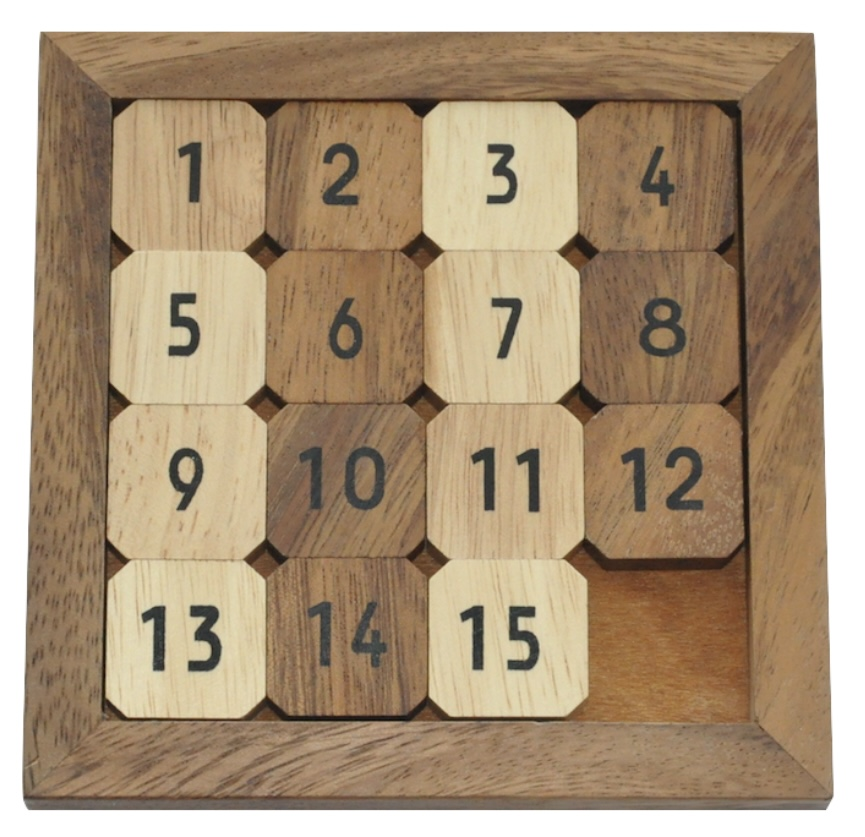
\includegraphics[width=0.25\linewidth]{images/15puzzle.jpg}
    \caption{The puzzle in its standard position.}
    \label{fig:toy}
\end{figure}

% \bigskip 
%     \begin{center}
%         \begin{tabular}{|c|c|c|c|}
%             \hline
%             1 & 2 & 3 & 4\\
%             \hline
%             5 & 6 & 7 & 8\\
%             \hline
%             9 & 10 & 11 & 12\\
%             \hline
%             13 & 14 & 15 & \\
%             \hline
%         \end{tabular}
%     \end{center}
% \bigskip 

The squares can slide vertically or horizontally using the empty square. Starting from the \emph{standard configuration}, 
namely the one shown in Figure~\ref{fig:toy}, one can reach any other \emph{admissible} position.
Around 1886, the following version of the puzzle (known as the \emph{(15,14)-puzzle}) 
became quite popular: Is the configuration 
\bigskip 
    \begin{center}
        \begin{tabular}{|c|c|c|c|}
            \hline
            1 & 2 & 3 & 4\\
            \hline
            5 & 6 & 7 & 8\\
            \hline
            9 & 10 & 11 & 12\\
            \hline
            13 & 15 & 14 & \\
            \hline
        \end{tabular}
    \end{center}
\bigskip 
admissible? In other words, can the puzzle be solved and moved to the standard configuration? 


A famous puzzle maker was so confident that the problem was very difficult 
that he even offered a substantial amount of money—\$1,000 at the time, which was a small fortune. 
The 15-puzzle has no solution. Let us see why.
We identity the configuration 
\bigskip 
    \begin{center}
        \begin{tabular}{|c|c|c|c|}
            \hline
            $\sigma_1$ & $\sigma_2$ & $\sigma_3$ & $\sigma_4$\\
            \hline
            $\sigma_5$ & $\sigma_6$ & $\sigma_7$ & $\sigma_8$\\
            \hline
            $\sigma_9$ & $\sigma_{10}$ & $\sigma_{11}$ & $\sigma_{12}$\\
            \hline
            $\sigma_{13}$ & $\sigma_{14}$ & $\sigma_{15}$ & $\sigma_{16}$\\
            \hline
        \end{tabular}
    \end{center}
\bigskip 
with the permutation $\sigma\in\Sym_{16}$ such that  
$\sigma(i)=\sigma_i$ for all $i\in\{1,\dots,16\}$. Here $\sigma_{16}$ 
represents the empty square. What happens to our permutation 
$\sigma$ when we move squares? It should be enough to see 
this in a concrete example. We know that the (15,14)-puzzle has
permutation $\sigma=(14\,15)$. Now if 
we move 12 down, then the resulting 
configuration is 
\bigskip 
    \begin{center}
        \begin{tabular}{|c|c|c|c|}
            \hline
            1 & 2 & 3 & 4\\
            \hline
            5 & 6 & 7 & 8\\
            \hline
            9 & 10 & 11 & \\
            \hline
            13 & 15 & 14 & 12\\
            \hline
        \end{tabular}
    \end{center}
\bigskip 
so the resulting permutation 
is $\sigma(12\,16)$. 

In general, moving squares correspond to multiplying  
our permutation by transpositions of the form $(i\,16)$ for
some $i\in\{1,\dots,15\}$. This means that 
after performing $m$ movements, 
one gets a configuration with 
permutation
\[
\tau_m\tau_{m-1}\cdots\tau_2\tau_1,
\]
where $\tau_1,\dots,\tau_m$ are transpositions. In particular, 
to ``solve'' the puzzle (that is, to return it into the default position), 
an even number of 
movements is needed. This explains why the puzzle cannot
be solved! 

\begin{bonus}
\label{xca:15tricky}
    Can you solve the following variant of the
    15-puzzle?

    \bigskip 
    \begin{center}
        \begin{tabular}{|c|c|c|c|}
            \hline
            \textsf{m} & \textsf{i} & \textsf{n} & \textsf{d}\\
            \hline
            \textsf{y} & \textsf{o} & \textsf{u} & \textsf{r}\\
            \hline
            \textsf{s} & \textsf{t} & \textsf{e} & \textsf{p}\\
            \hline
            \textsf{n} & \textsf{w} & \textsf{o} & \\
            \hline
        \end{tabular}
    \end{center}
    \bigskip 
\end{bonus}